\documentclass{standalone}
\usepackage{tikz}
\usetikzlibrary{patterns}
\usetikzlibrary{positioning}
\usetikzlibrary{patterns, positioning}
\usetikzlibrary{shapes.misc}
\usepackage[outline]{contour}
\contourlength{1.5pt} 
\usepackage[sfdefault]{ClearSans}

\begin{document}
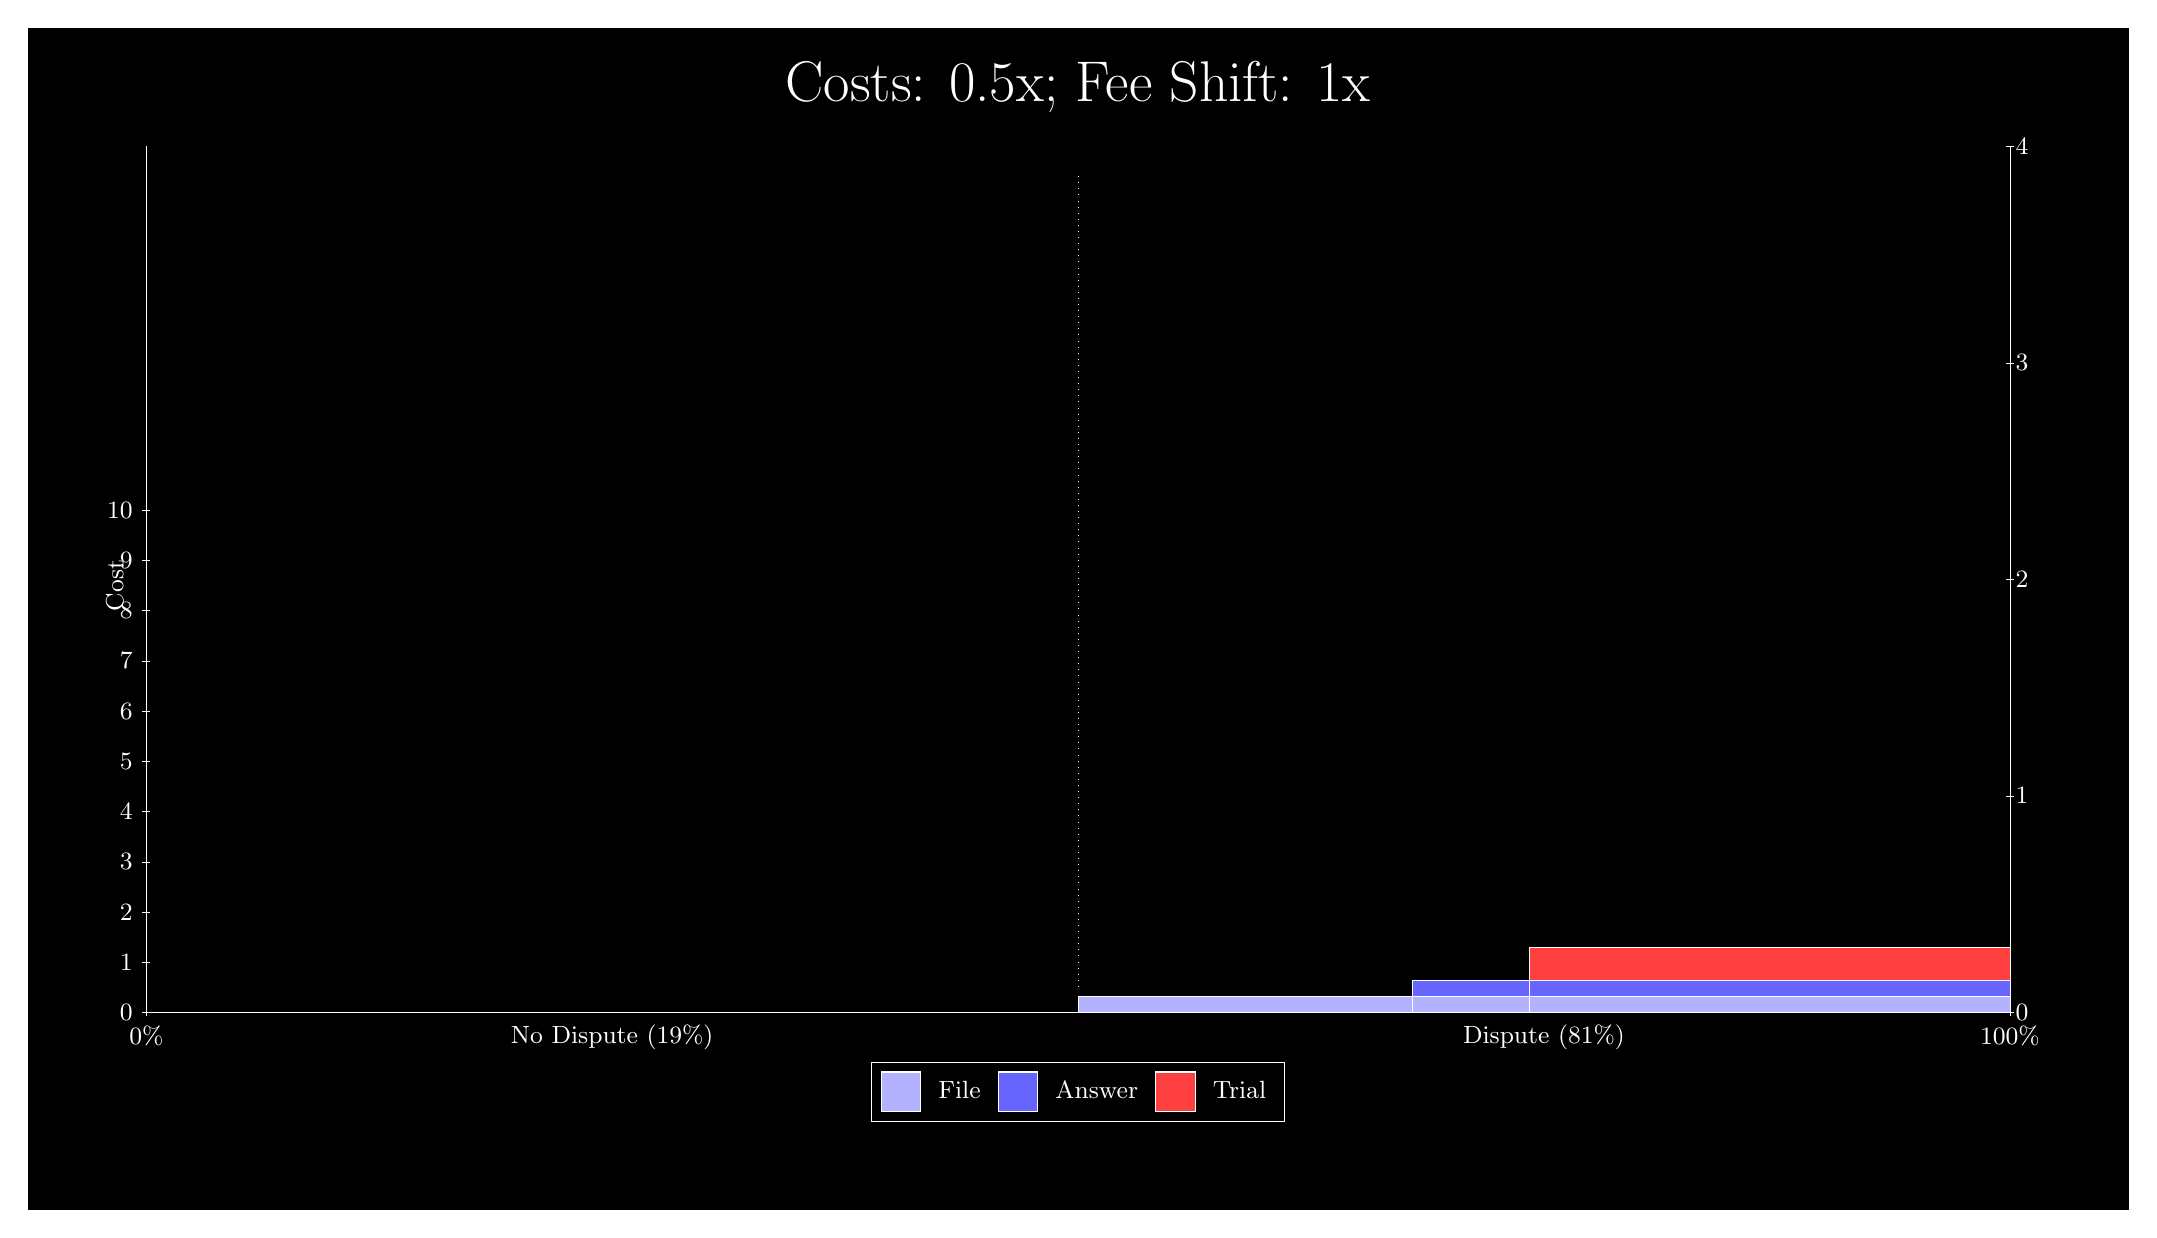
\begin{tikzpicture}
\draw[fill=black] (0,0) rectangle (26.667,15);
\draw[draw=none,text=white] (0,13.5) rectangle (26.667,15) node[midway] {\huge Costs: 0.5x; Fee Shift: 1x };
\draw[fill=blue!30,draw=white,very thin] (13.333,2.5) rectangle (17.582,2.7063);
\draw[fill=blue!30,draw=white,very thin] (17.582,2.5) rectangle (19.061,2.7063);
\draw[fill=blue!60,draw=white,very thin] (17.582,2.7063) rectangle (19.061,2.9125);
\draw[fill=blue!30,draw=white,very thin] (19.061,2.5) rectangle (25.167,2.7063);
\draw[fill=blue!60,draw=white,very thin] (19.061,2.7063) rectangle (25.167,2.9125);
\draw[fill=red!75,draw=white,very thin] (19.061,2.9125) rectangle (25.167,3.325);
\draw[white,very thin] (1.5,2.5) -- (1.5,13.5);
\node[font=\small,rotate=90,text=white, anchor=center] at (1.1, 7.9222) {Cost};
\draw[white,very thin] (1.45,2.5) -- (1.55,2.5);
\node[font=\small,text=white, anchor=east] at (1.45, 2.5) {0};
\draw[white,very thin] (1.45,3.1379) -- (1.55,3.1379);
\node[font=\small,text=white, anchor=east] at (1.45, 3.1379) {1};
\draw[white,very thin] (1.45,3.7758) -- (1.55,3.7758);
\node[font=\small,text=white, anchor=east] at (1.45, 3.7758) {2};
\draw[white,very thin] (1.45,4.4137) -- (1.55,4.4137);
\node[font=\small,text=white, anchor=east] at (1.45, 4.4137) {3};
\draw[white,very thin] (1.45,5.0516) -- (1.55,5.0516);
\node[font=\small,text=white, anchor=east] at (1.45, 5.0516) {4};
\draw[white,very thin] (1.45,5.6895) -- (1.55,5.6895);
\node[font=\small,text=white, anchor=east] at (1.45, 5.6895) {5};
\draw[white,very thin] (1.45,6.3275) -- (1.55,6.3275);
\node[font=\small,text=white, anchor=east] at (1.45, 6.3275) {6};
\draw[white,very thin] (1.45,6.9654) -- (1.55,6.9654);
\node[font=\small,text=white, anchor=east] at (1.45, 6.9654) {7};
\draw[white,very thin] (1.45,7.6033) -- (1.55,7.6033);
\node[font=\small,text=white, anchor=east] at (1.45, 7.6033) {8};
\draw[white,very thin] (1.45,8.2412) -- (1.55,8.2412);
\node[font=\small,text=white, anchor=east] at (1.45, 8.2412) {9};
\draw[white,very thin] (1.45,8.8791) -- (1.55,8.8791);
\node[font=\small,text=white, anchor=east] at (1.45, 8.8791) {10};

\draw[white,dotted,very thin] (13.333,2.83) -- (13.333,13.17);
\draw[white,very thin] (25.167,2.5) -- (25.167,13.5);
\draw[white,very thin] (25.117,2.5) -- (25.217,2.5);
\node[font=\small,text=white, anchor=west] at (25.117, 2.5) {0};
\draw[white,very thin] (25.117,5.25) -- (25.217,5.25);
\node[font=\small,text=white, anchor=west] at (25.117, 5.25) {1};
\draw[white,very thin] (25.117,8) -- (25.217,8);
\node[font=\small,text=white, anchor=west] at (25.117, 8) {2};
\draw[white,very thin] (25.117,10.75) -- (25.217,10.75);
\node[font=\small,text=white, anchor=west] at (25.117, 10.75) {3};
\draw[white,very thin] (25.117,13.5) -- (25.217,13.5);
\node[font=\small,text=white, anchor=west] at (25.117, 13.5) {4};

\draw[white,very thin] (1.5,2.5) -- (25.167,2.5);
\draw[white,very thin] (1.5,2.45) -- (1.5,2.55);
\node[font=\small,text=white, anchor=north] at (1.5, 2.45) {0\%};
\draw[white,very thin] (25.167,2.45) -- (25.167,2.55);
\node[font=\small,text=white, anchor=north] at (25.167, 2.45) {100\%};

\node[font=\small,text=white,anchor=south] at (7.4167, 1.9) {No\ Dispute\ (19\%)};
\node[font=\small,text=white,anchor=south] at (19.25, 1.9) {Dispute\ (81\%)};
\draw (13.3333,2.5) node (B) {};
\begin{scope}[align=center]
\matrix[scale=0.5,draw=white,below=0.5cm of B,nodes={draw},column sep=0.1cm]{
\node[rectangle,draw,minimum width=0.5cm,minimum height=0.5cm,fill=blue!30]{}; & \node[draw=none,font=\small,text=white]{File}; &
\node[rectangle,draw,minimum width=0.5cm,minimum height=0.5cm,fill=blue!60]{}; & \node[draw=none,font=\small,text=white]{Answer}; &
\node[rectangle,draw,minimum width=0.5cm,minimum height=0.5cm,fill=red!75]{}; & \node[draw=none,font=\small,text=white]{Trial}; \\\\
};\end{scope}

\end{tikzpicture}
\end{document}